% Lecture Template for ME3050-001-002-Tristan Hill - Spring 2020
% Dynamics Modeling and Controls
% Frequency Response

% I am finally converting my stuff to BEAMER

% Document settings

%\documentclass{beamer}                  % for presentation ?
\documentclass[handout]{beamer}  % for handout ?
\usepackage{beamerthemesplit}
\usepackage{amsmath}
\usepackage{listings}
\usepackage{multicol}
\usepackage{framed}
\usepackage{amssymb}


\lstdefinestyle{myCustomMatlabStyle}{
  language=Matlab,
  numbers=left,
  stepnumber=1,
  numbersep=10pt,
  tabsize=4,
  showspaces=false,
  showstringspaces=false
}
\lstset{basicstyle=\ttfamily\tiny,style=myCustomMatlabStyle}
%lstset{language=MATLAB,basicstyle=\ttfamily\small,showstringspaces=false}



\beamertemplateballitem

\definecolor{TTUpurple}{rgb}{0.3098, 0.1607, 0.5176} % TTU Purple (primary)
\definecolor{TTUgold}{rgb}{1.0000, 0.8666, 0.0000} % TTU Gold (primary)

\setbeamercolor{palette primary}{bg=TTUpurple,fg=TTUgold}
\setbeamercolor{palette secondary}{bg=black,fg=TTUgold}
\setbeamercolor{palette tertiary}{bg=black,fg=TTUpurple}
\setbeamercolor{palette quaternary}{bg=TTUgold,fg=black}
\setbeamercolor{structure}{fg=TTUpurple} % itemize, enumerate, etc
\setbeamercolor{section in toc}{fg=TTUpurple} % TOC sections

%\DeclareSymbolFont{bbold}{U}{bbold}{m}{n}
%\DeclareSymbolFontAlphabet{\mathbbold}{bbold}

%\newcommand{\bbfamily}{\fontencoding{U}\fontfamily{bbold}\selectfont}
%\DeclareMathAlphabet{\mathbbold}{U}{bbold}{m}{n}

%\usefonttheme{professionalfonts}

\newcommand{\vspccc}{\vspace{6mm}\\} % large vertical space
\newcommand{\vspcc}{\vspace{4mm}\\}   % medium vertical space
\newcommand{\vspc}{\vspace{2mm}\\}     % small vertical space

\newcommand{\hspcccc}{\hspace{10mm}} % large horizontal space
\newcommand{\hspccc}{\hspace{6mm}} % large horizontal space
\newcommand{\hspcc}{\hspace{4mm}}   % medium horizontal space
\newcommand{\hspc}{\hspace{2mm}}     % small horizontal space


\newcommand{\LT}{\mathcal{L}} % lagrangian

\newcommand{\LNUM}{3 } %Lecture number 2

\newcommand{\secondtitle}{Frequency Response of 2$^{nd}$ Order Systems}% second line of the title of this presentation , aka the topic of this lecture

\title{Frequency Response - Lecture \LNUM}
\author{ME3050 - Dynamics Modeling and Controls} % original formatting from Mike Renfro, September 21, 2004

\date{April  25, 2020}

\begin{document}

\lstset{language=MATLAB,basicstyle=\ttfamily\small,showstringspaces=false}

% Title page1 
\frame{\titlepage \center\textbf{\secondtitle}\vspcc}


% Section 0: Outline
\frame{

\large \textbf{Lecture \LNUM - \secondtitle} \vspc

 \begin{itemize}

	\item Review Transfer Functions\vspc % Section 1: 

	\item Frequency Response of Overdamped Systems\vspc % Section 2
	
	\item Frequency Response of Underdamped Systems\vspc %Section 3

	\item MATLAB code for Bode Plots \vspc %Section 3
%\item Graph of Frequency Response in MATLAB\vspace{2mm} % Section 4

\end{itemize}

}


%Section 1: Review Transfer Functions
\section{Review Transfer Functions}

\subsection{Equivalent System Representations}
\frame{
\frametitle{Equivalent System Representations}

\small 
The{\bf Transfer Function} is the input-output relationship in the frequency domain and can be found from the equation of motion of the system.\vspcc 

\scalebox{1.25}{$T(s)=\frac{X(s)}{F(s)}$}\vspcc

The Transfer Function is an equivalent representation of the system. \vspcc
\begin{framed}
\scalebox{1.25}{E.O.M$\hspace{5mm} \leftrightarrow \hspace{5mm}$ T(s)$\hspace{5mm} \leftrightarrow \hspace{5mm}$ Block Diagram}\\
\end{framed}

}

\subsection{Transfer Function of 2$^{nd}$ Order System}
\frame{
\frametitle{Transfer Function of 2$^{nd}$ Order System}

\scalebox{1}{$m\ddot{x}+c\dot{x}+kx=f(t)$ \hspace{5mm}with\hspace{5mm} $f(t)=Asin(\omega t)$} \vspcc
The transfer function can easily be found by taking the Laplace transform of the equation of motion. \vspcc

\begin{framed}
\scalebox{1}{$T(s)=\frac{X(s)}{F(s)}=\frac{1}{ms^2+cs+k}$ \hspace{5mm} Second Order Transfer Function} \vspc
\end{framed}

}

% section 2: Frequency Response of Overdamped Systems

\section{Frequency Response of Overdamped Systems}

\subsection{The Overdamped System}
\frame{
\frametitle{The Overdamped System}

\small

In an \underline{overdamped} system, both roots are real and distinct.\vspcc
The transfer function is shown below in terms of the system parameters\vspc

\scalebox{1.0}{$T(s)=\frac{X(s)}{F(s)}=\frac{1/k}{\left(\frac{m}{k}\right)s^2+\left(\frac{c}{k}\right)s+1}=\frac{1/k}{(\tau_1 s+1)(\tau_2 s+1)} \hspace{5mm} \tau_1,\tau_2$ - time constants}\vspc

Substitute $s=j\omega$ into the transfer function and find the amplitude ratio and phase angle.\vspc

\scalebox{1.0}{$T(s) \rightarrow T(j\omega) =\frac{1/k}{\left(\tau_1j\omega+1\right)\left(\tau_1j\omega+1\right)}$}\vspc

\begin{framed}
\scalebox{1}{$M\left(\omega\right)=|T\left(j\omega\right)|=\frac{|1/k|}{|\tau_1j\omega+1||\tau_2j\omega+1|}$} \vspc
\scalebox{1}{$m\left(\omega\right)=20logM\left(\omega\right)=20log|1/k|-20log|\tau_1\omega j+1|-20log|\tau_2\omega j+1|$}\vspc
\scalebox{1}{$\phi\left(\omega\right)=\angle\frac{1}{k}-\angle\left(\tau_1\omega j+1\right)-\angle\left(\tau_2\omega_j+1\right)$}
\end{framed}
}

\subsection{The Bode Diagram }
\frame{
\frametitle{The Bode Diagram}
\small
These three terms can be seen on the Bode diagram. \vspc
\scalebox{1}{$m\left(\omega\right)=20logM\left(\omega\right)=20log|1/k|-20log|\tau_1\omega j+1|-20log|\tau_2\omega j+1|$}\vspc

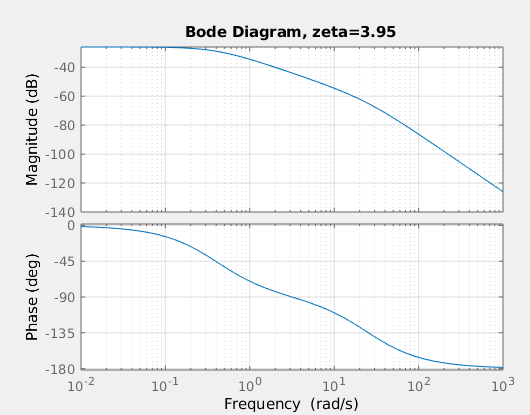
\includegraphics[scale=.30]{lecture3_fig3.png}

This shows that the magnitude ratio of the system across different regions of the input frequency. 

}

% section 3: Frequency Response of Underdamped Systems

\section{Frequency Response of Underdamped Systems}

\subsection{The Underdamped System}
\frame{
\frametitle{The Underdamped System}

\small

In an \underline{underdamped} system, the roots are complex conjugates.\vspcc
The transfer function is shown below in terms of the system parameters\vspc

\scalebox{1.0}{$T(s)=\frac{X(s)}{F(s)}=\frac{1/k}{\left(\frac{m}{k}\right)s^2+\left(\frac{c}{k}\right)s+1}=\frac{1/k}{\left(\frac{s}{\omega_n}\right)^2+2\zeta\left(\frac{s}{\omega_n}\right)+1}$} \vspc
\scalebox{1.0}{$T(s)=\frac{kX(s)}{F(s)}=\frac{\omega_n^2}{s^2+2\zeta\omega_ns+\omega_n^2}$}\vspc

Notice we factored out $k$ to form the ratio of output displacement $X(s)$ to input displacement $\frac{F(s)}{k}$. You can see this with Hooke's Law $F=kx\implies x=\frac{F}{k}$. \vspc

This also allows us to define the transfer function in terms of $\zeta$ and $\omega_n$. Substitue $s=j\omega$ and mulitply the equation $\frac{1/\omega_n^2}{1/\omega_n^2}$.
\scalebox{1.0}{$T(s)\rightarrow T(j\omega)=\frac{1}{\left(\frac{j\omega}{\omega_n}\right)^2+\left(\frac{2\zeta}{\omega_n}\right)j\omega+1}=\frac{1}{1-\left(\frac{\omega}{\omega_n}\right)^2+\left(\frac{2\zeta\omega}{\omega_n}\right)j}$} \vspc
}


\subsection{The Frequency Ratio}
\frame{
\frametitle{The Frequency Ratio}

\small 

To simplify this expression we define another new quantity the frequency ratio, $r$ as the ratio of input frequency to natural frequency of the system. The transfer function is re-written in terms of the frequency ratio. \vspc

\scalebox{1.0}{$r=\frac{\omega}{\omega_n} \hspc\rightarrow\hspc T\left(j\omega\right) \hspc\rightarrow\hspc T\left(r\right)=\frac{1}{1-r^2+2\zeta rj}$} \vspcc

Now the amplitude ratio and phase are written in tems of $r$. \vspcc

\begin{framed}
\scalebox{1}{$M=|T\left(r\right)|=\frac{1}{\sqrt{\left(1-r^2\right)^2+\left(2\zeta r\right)^2}}$}\vspc
\scalebox{1}{$\implies m=20logM=-10log\left[\left(1-r^2\right)^2+\left(2\zeta r\right)^2\right]$} \vspcc
\scalebox{1}{$\phi=\angle 1 - \angle\left(1-r^2+2\zeta rj\right)\implies \phi=-tan\left(\frac{2\zeta r}{1-r^2}\right)$}\vspc
\end{framed}

}

\subsection{The Bode Diagram }
\frame{
\frametitle{The Bode Diagram}
\small

In the underdamped second order system only two regions are present in the Bode diagram. 

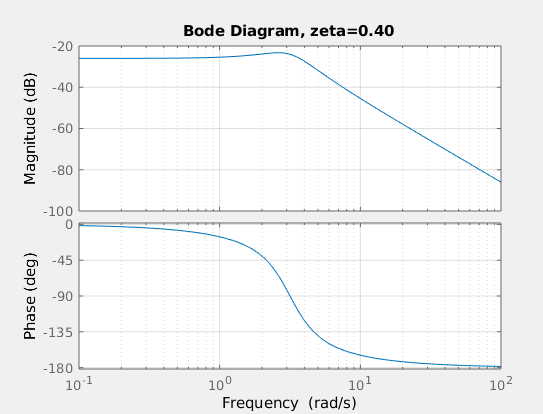
\includegraphics[scale=.27]{lecture3_fig4.png}  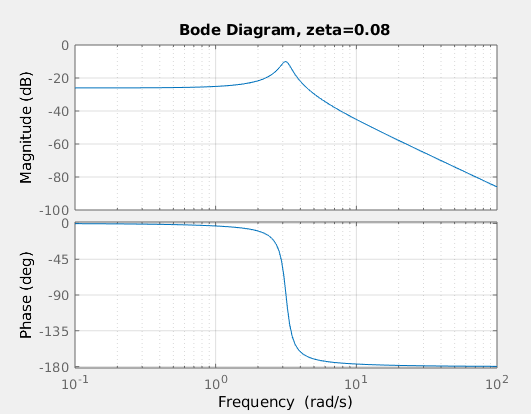
\includegraphics[scale=.27]{lecture3_fig5.png} 

As the damping ratio decreases something significant happens. This Bode diagram shows something that the others before have not.

}

% section 4: Bode Plots in MATLAB
\frame[containsverbatim]{
\frametitle{Bode Plots in MATLAB}

Vary the system parameter in the scripts to make the plots shown. 

\begin{lstlisting}
clear variables;clc;close all

% define the system parameters
m=2;c=1;k=20;
zeta=c/(2*sqrt(m*k));

% create a system object from the transfer function
sys=tf(1/k,[(m/k) (c/k) 1]);

% use built-in MATLAB Bode Plot
figure(1)

bode(sys);grid on
str=sprintf('Bode Diagram, zeta=%.2f',zeta);
title(str)
\end{lstlisting}

}

% references is not a section for now, for looks and it would be a waste of space
\frame{

\frametitle{References}

\begin{itemize}
	\item System Dynamics, Palm III, Third Edition - Chapter 9 - System Response in the Frequency Domain
\end{itemize}

}

\end{document}









 